\subsection{API Gateway}

L'API Gateway è il cuore della piattaforma. Il suo compito è, previa verifica dei privilegi e aggiornamento del database SLA, reindirizzare le chiamate dell'utilizzatore finale e instradarle verso il fornitore del microservizio.  La necessità del passaggio per un gateway centralizzato sono per motivi di data analysis nonchè di controllo della validità delle chiavi.

L'API Gateway è parte del package di Back-end, tuttavia l'approccio a microservizi adottato ci consente di descriverlo come un entità a sè stante. Esso è composto dai campi dati per mantenere in coda le chiamate, e un servizio interno che si occupa di effettuare le operazioni di verifica chiave, verifica e scrittura SLA, forwarding delle chiamate e forwarding delle risposte. 

\subsubsection{APIM::BackEnd::APIGateway}

Il package principale per il servizio API Gateway è rappresentato dal seguente diagramma UML: 

\begin{figure}[!htbp]
	\centering
	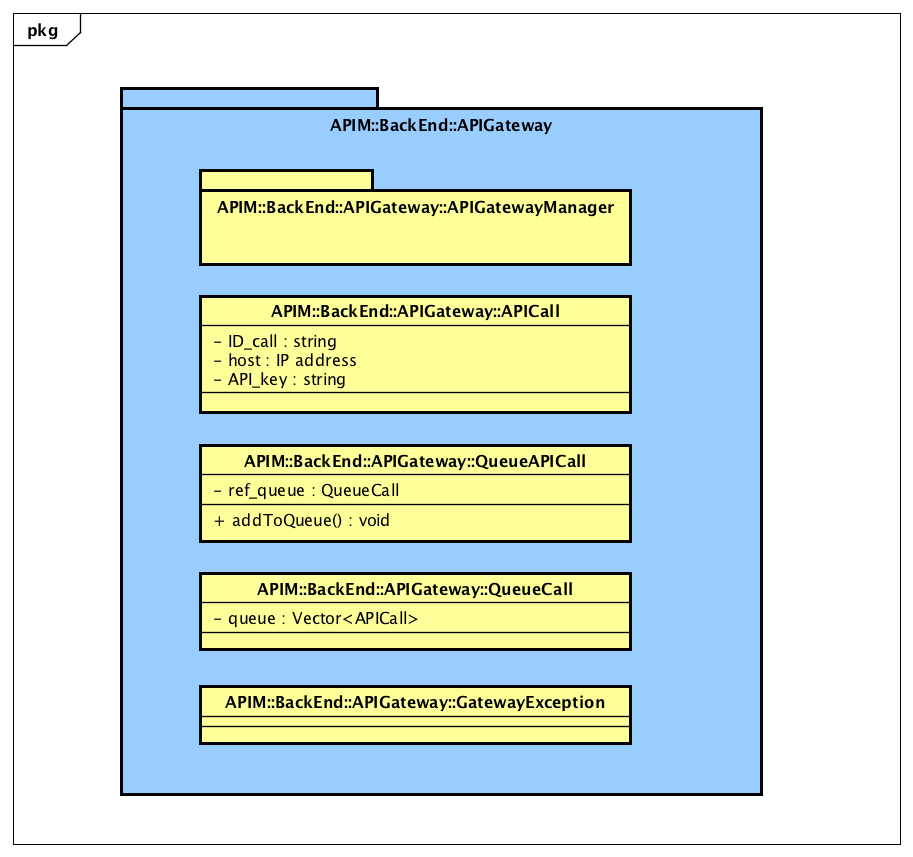
\includegraphics[scale=0.45]{UML/DiagrammiPackage/ApiGateway.png}
	\caption{ApiGateway}
\end{figure}



